\begin{document}
\chapter{ABIG}
This Supplementary Material provides additional derivations, implementation details and results. More specifically: 
\begin{itemize}[noitemsep]

    \item Section \ref{ap:method} proposes derivations, implementation details and analysis related to our method.
    \begin{itemize}[noitemsep]
        \item Subsection \ref{ap:sec_sketch} provides additional diagrams illustrating the ABP problem and its position with respect to related settings.
        \item Subsection \ref{ap:method_analytic} proposes the full derivation of the agents' MDP.
        \item Subsection \ref{ap:algo} proposes our methods pseudo-code, algorithmic implementation details (for BC and MCTS), hyper-parameters and compute resources.
        \item Subsection \ref{sup:sec_res_toy} proposes analysis that explore our method's learning mechanisms.
        \item Subsection \ref{ap:sec_related_work} discusses the differences between \abp and Hierarchical/Feudal Reinforcement Learning.
    \end{itemize}
\end{itemize}

% % Add the appendix text to the document TOC
% \part{\textsc{Supplementary Material}} % Start the appendix part
% \addcontentsline{toc}{paragraph}{Appendix}
% \parttoc % Insert the appendix TOC

\section{Supplementary Methods}
\label{ap:method}

\subsection{Supplementary Sketches}
\label{ap:sec_sketch}
\begin{figure}[h!]
    \centering
    \begin{tabular}{cc}
    \multicolumn{2}{c}{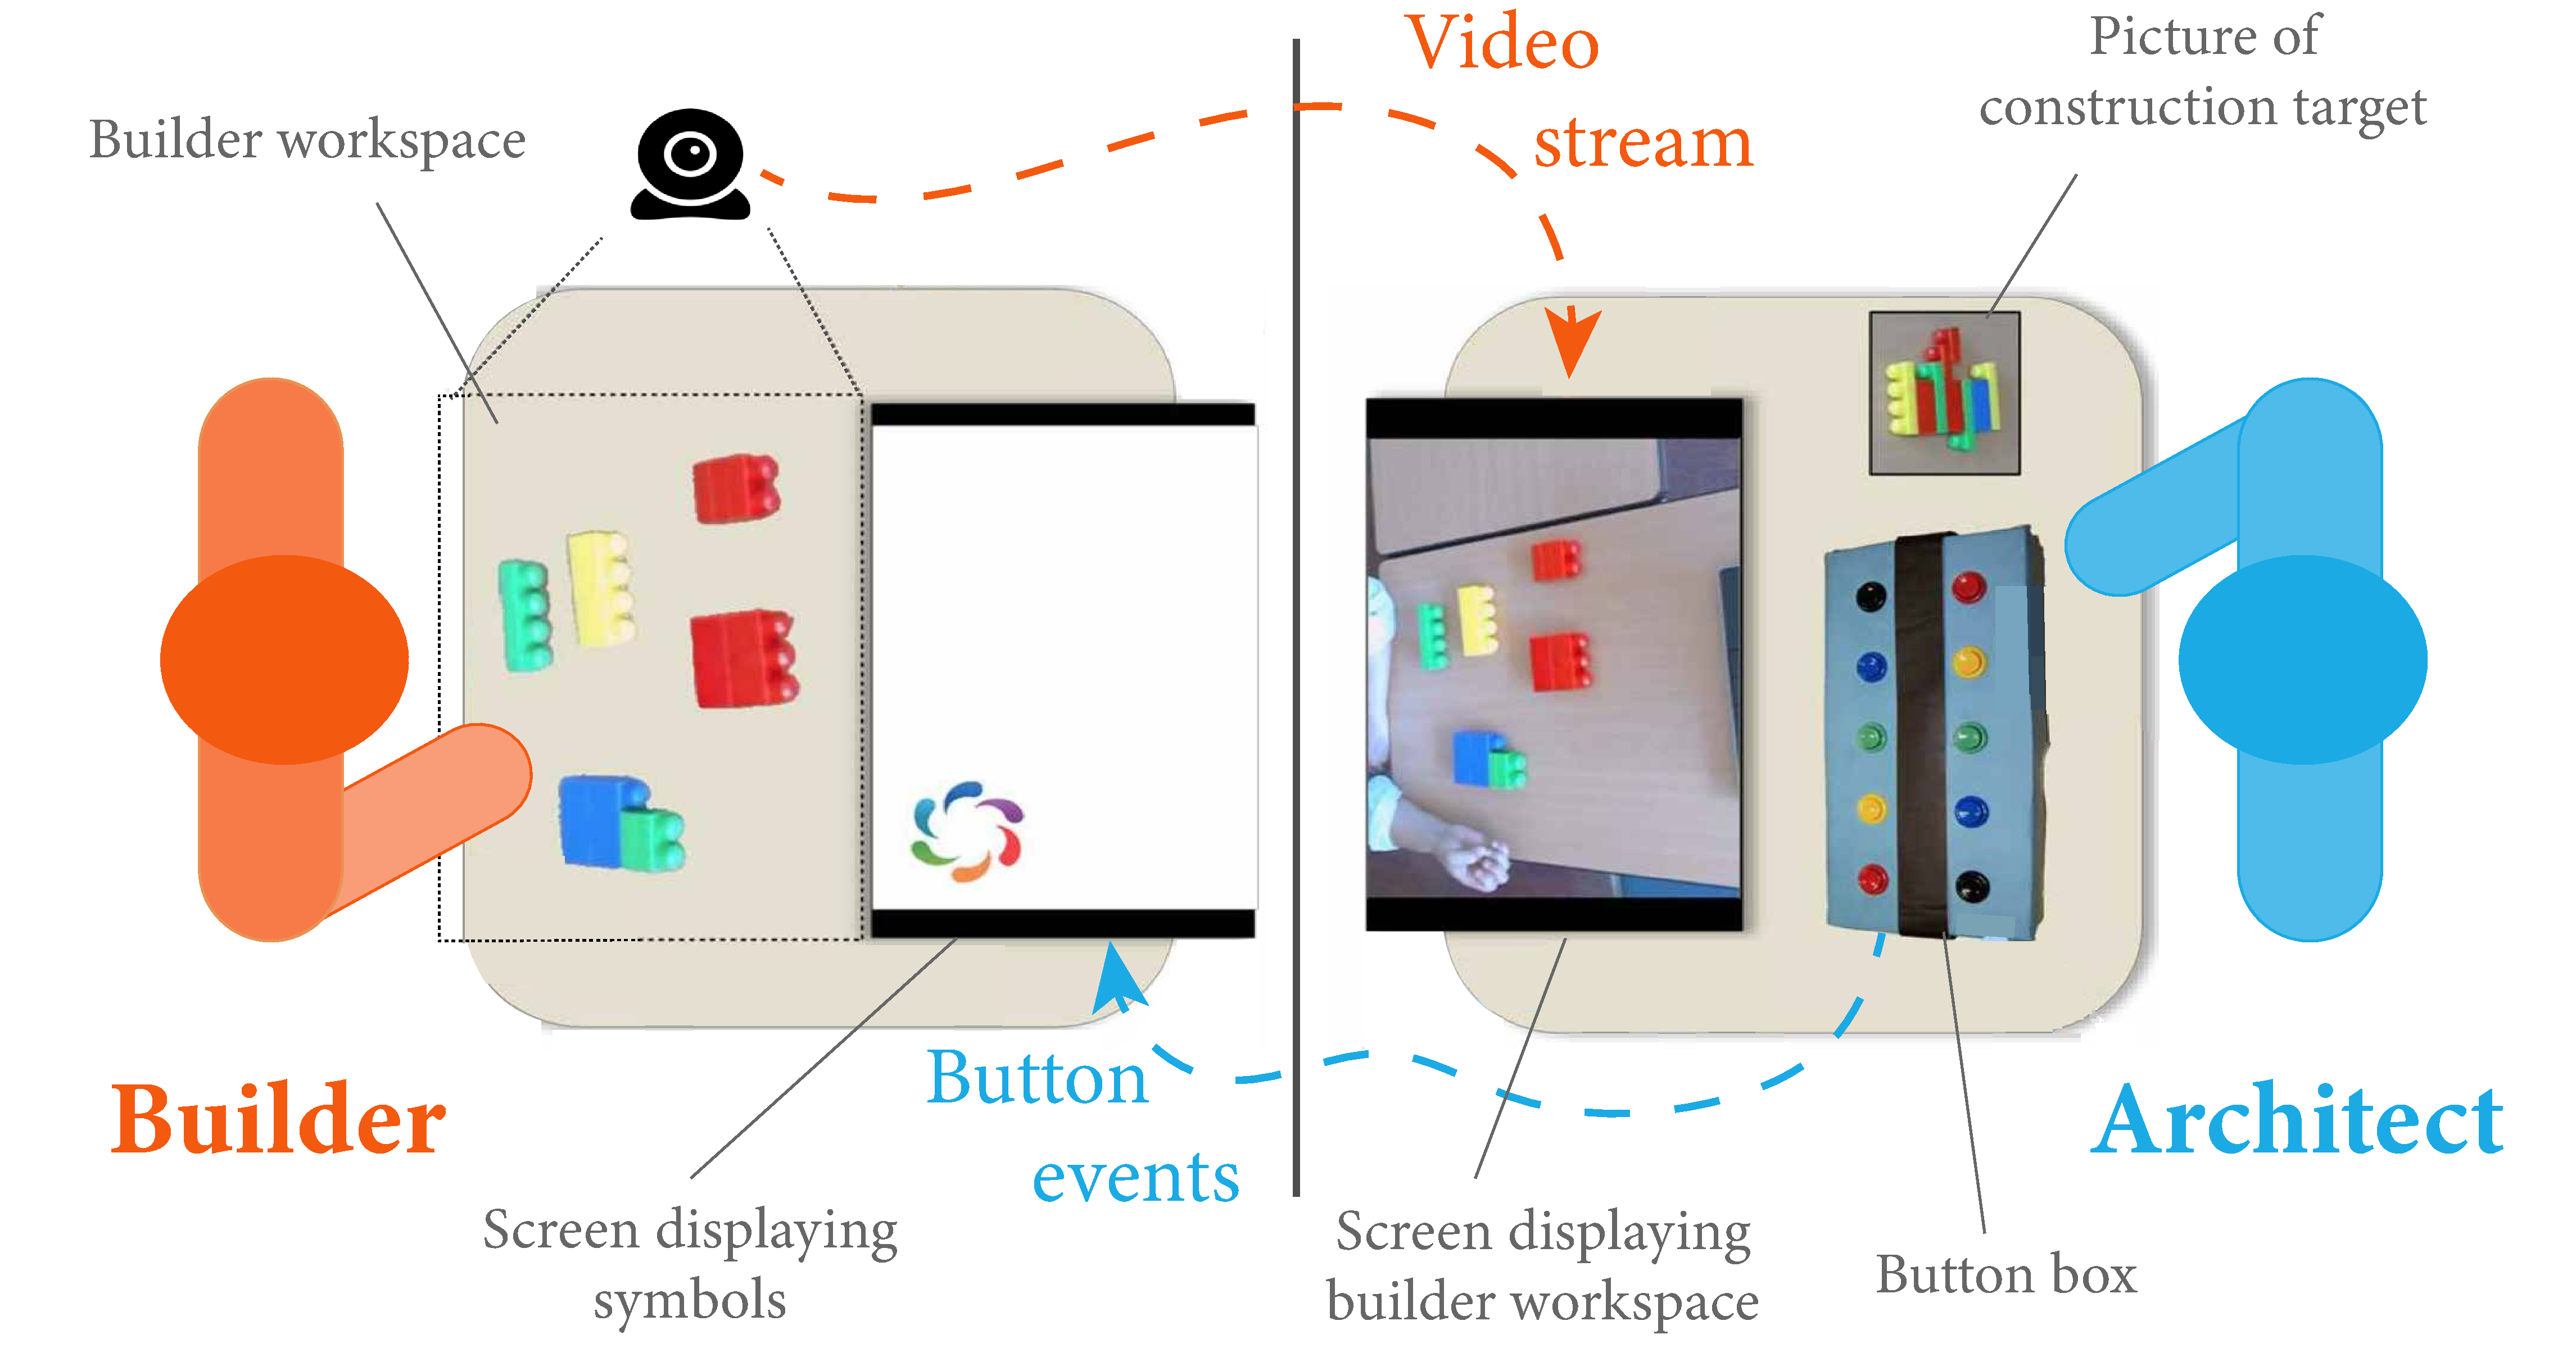
\includegraphics[width=0.5\textwidth]{abig/cocogame_horizontal.pdf}}\\
    \multicolumn{2}{c}{\small (a)}\\
 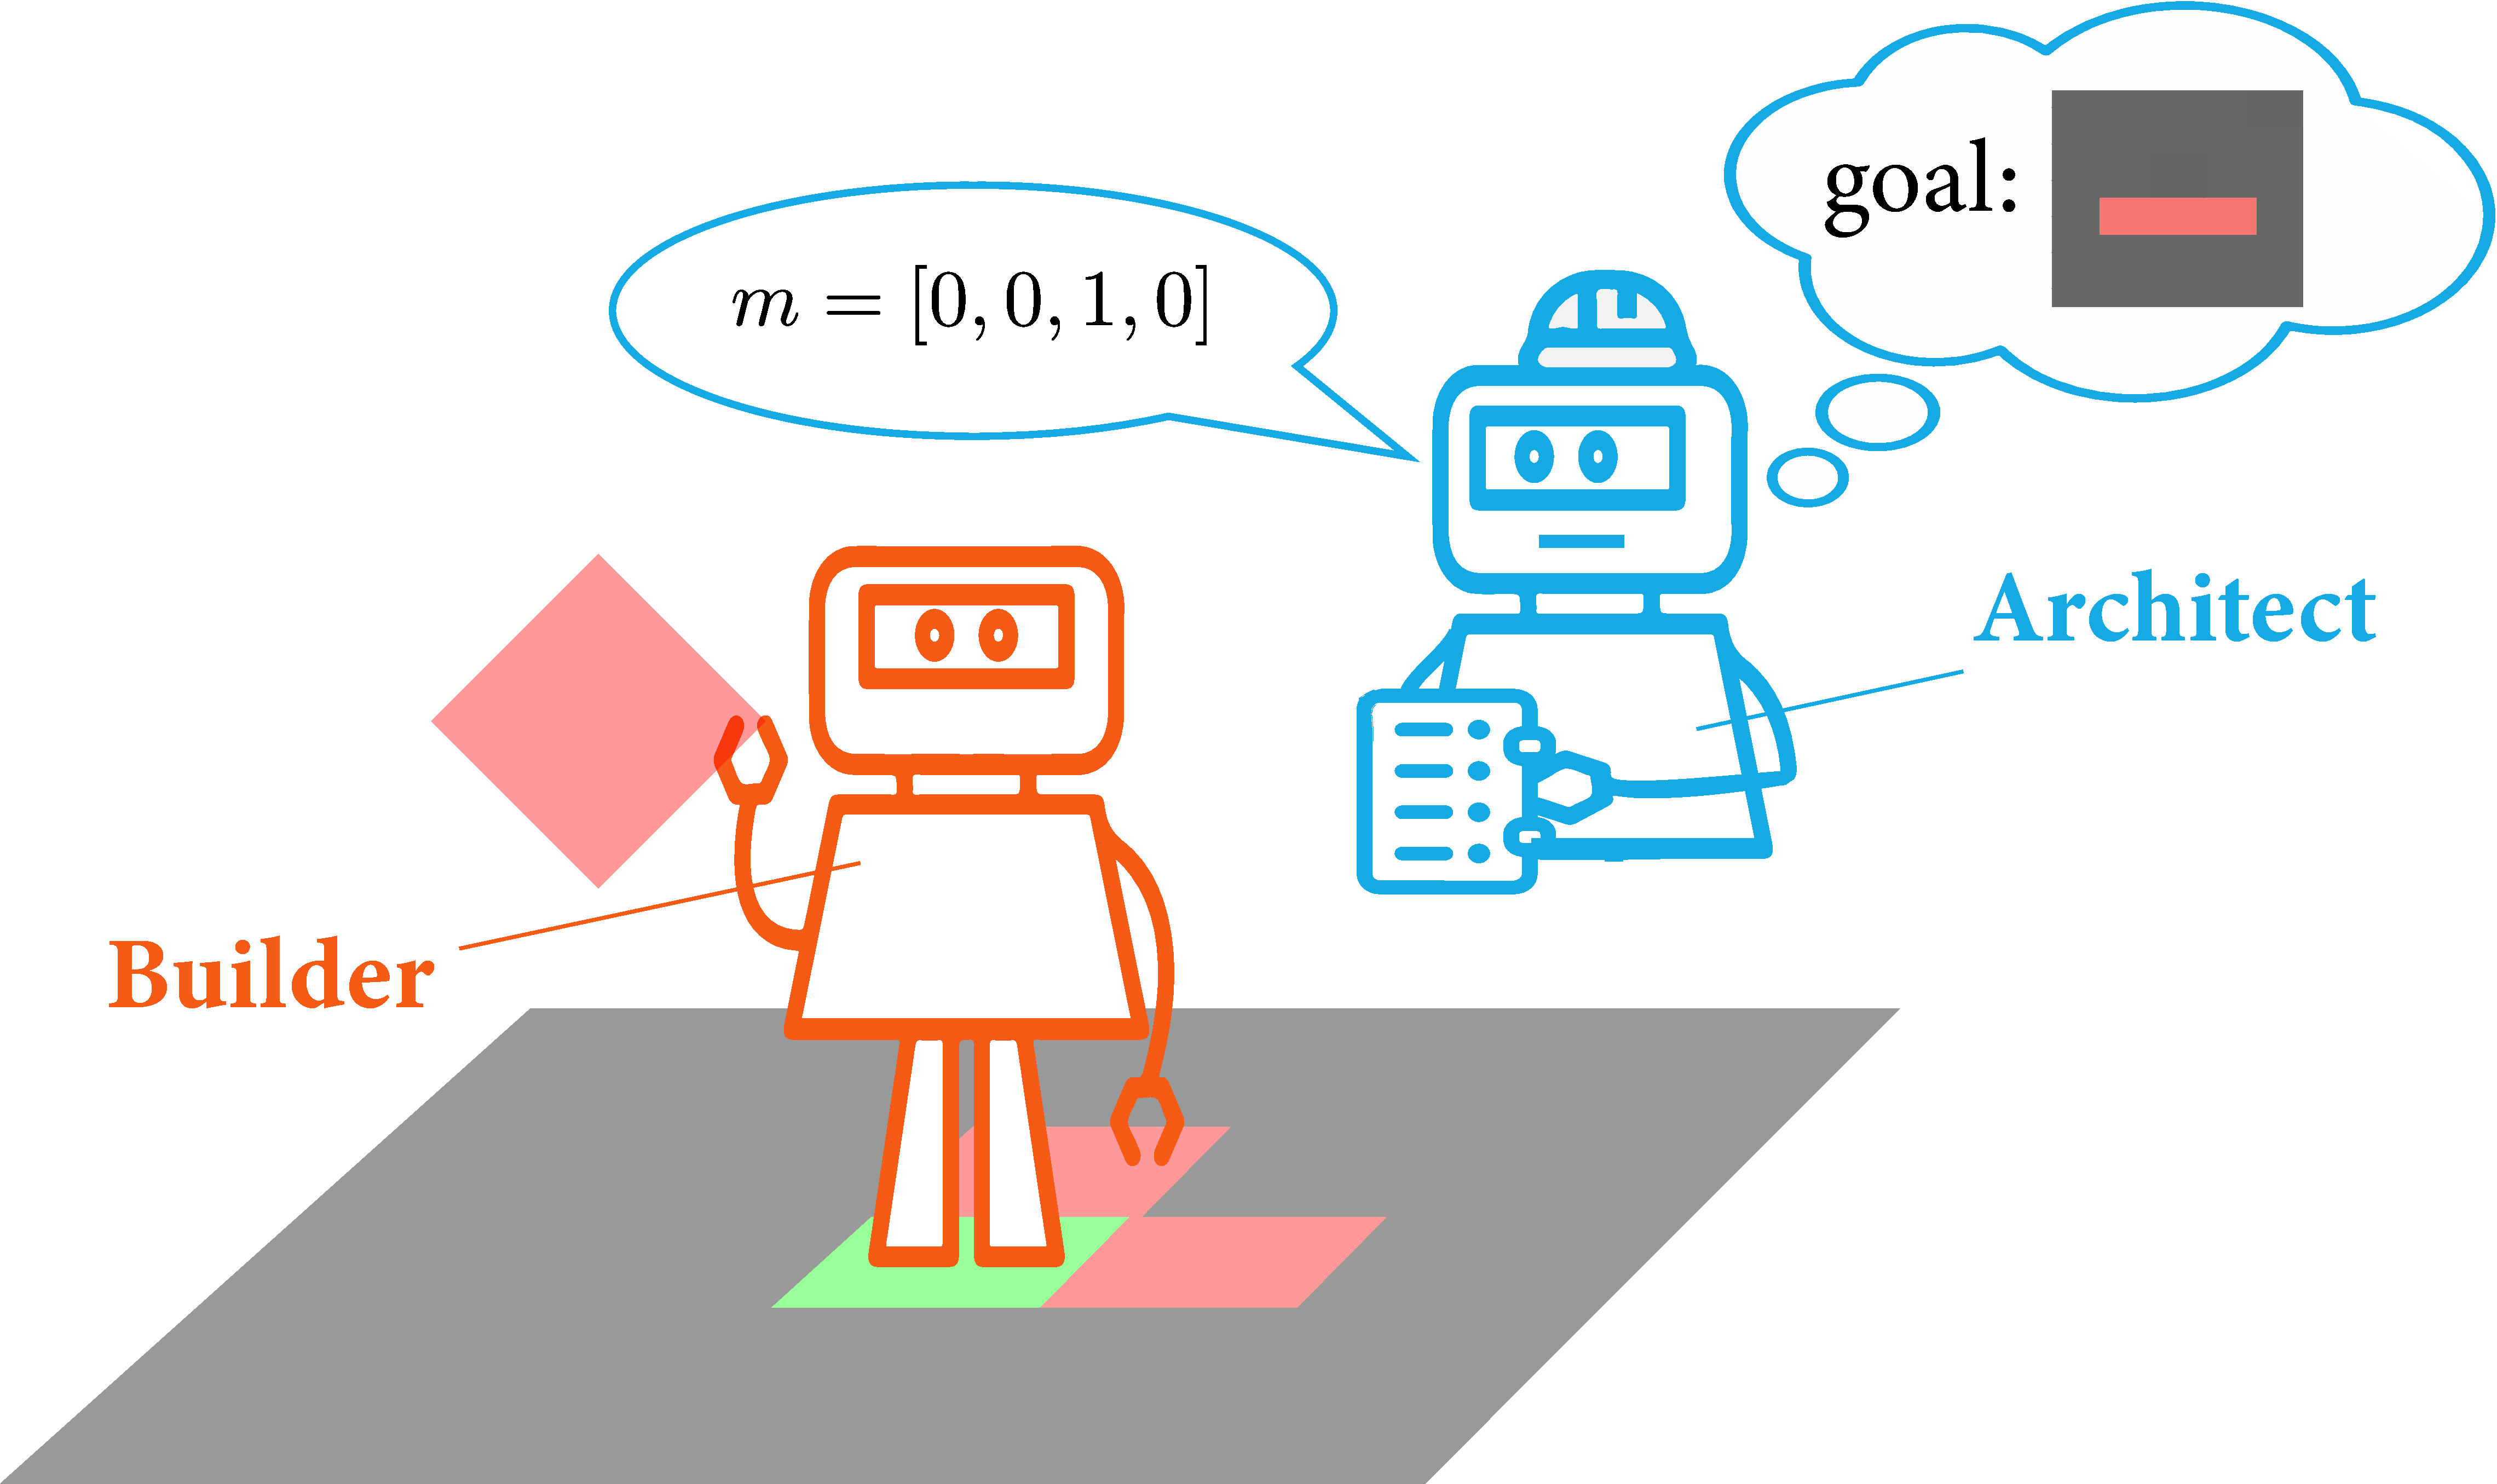
\includegraphics[width=0.45\textwidth]{abig/high_level_figure}    &  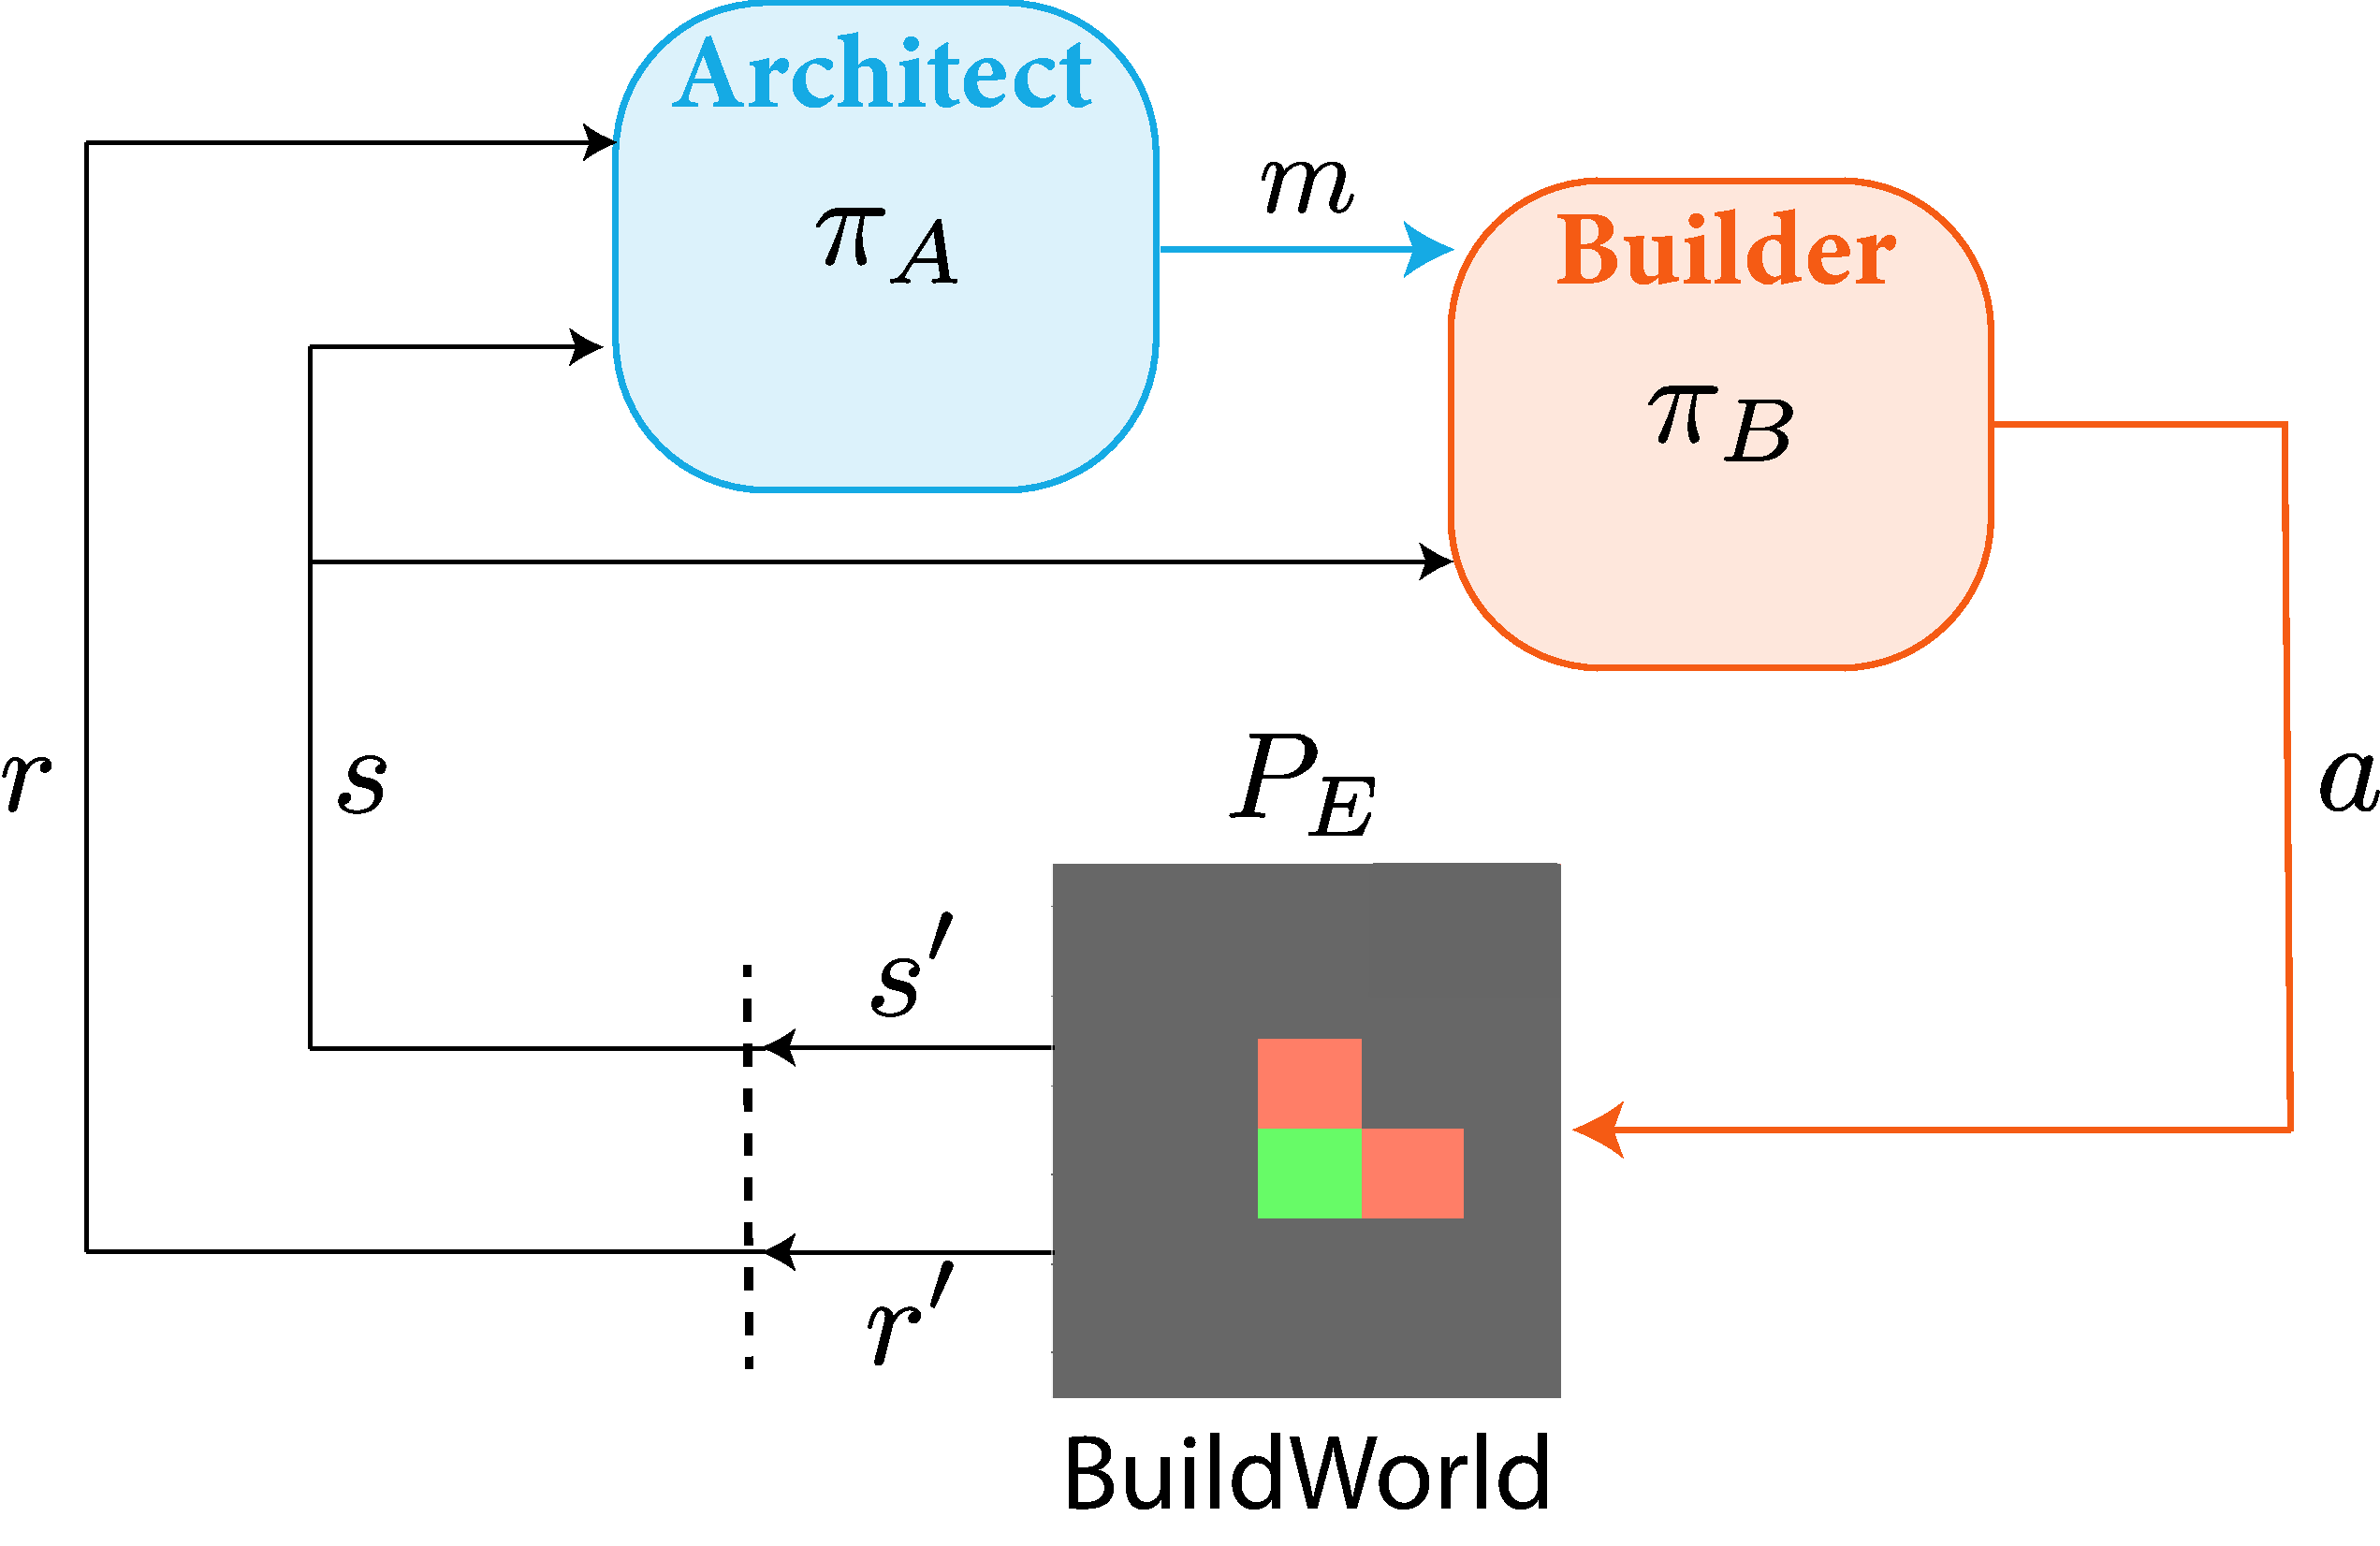
\includegraphics[width=0.4\textwidth]{abig/agent_diagram_v2} \\
    \small (b) & \small(c)
    \end{tabular}
    \caption{\small (a) \textbf{Schematic view of the CoCo Game.} The architect and the builder should collaborate in order to build the construction target while located in different rooms. The architecture has a picture of the target while the builder has access to the blocks. The architect monitors the builder workspace via a camera (video stream) and can communicate with the builder only through the use of 10 symbols (button events). (b) \textbf{Schematic view of the Architect-Builder Problem. } The architect must learn how to use messages to guide the builder while the builder needs to learn to make sense of the messages in order to be guided by the architect. (c) \textbf{Interaction diagram between the agents and the environment in our proposed \abp.} The architect communicates messages ($m$) to the builder.  Only the builder can act ($a$) in the environment. The builder conditions its action on the message sent by the builder ($\pib(a|s,m)$). The builder never perceives any reward from the environment}
    \label{fig:sup_diagram}
\end{figure}

\begin{figure}[h!]
    \centering
    \begin{tabular}{cccc}
    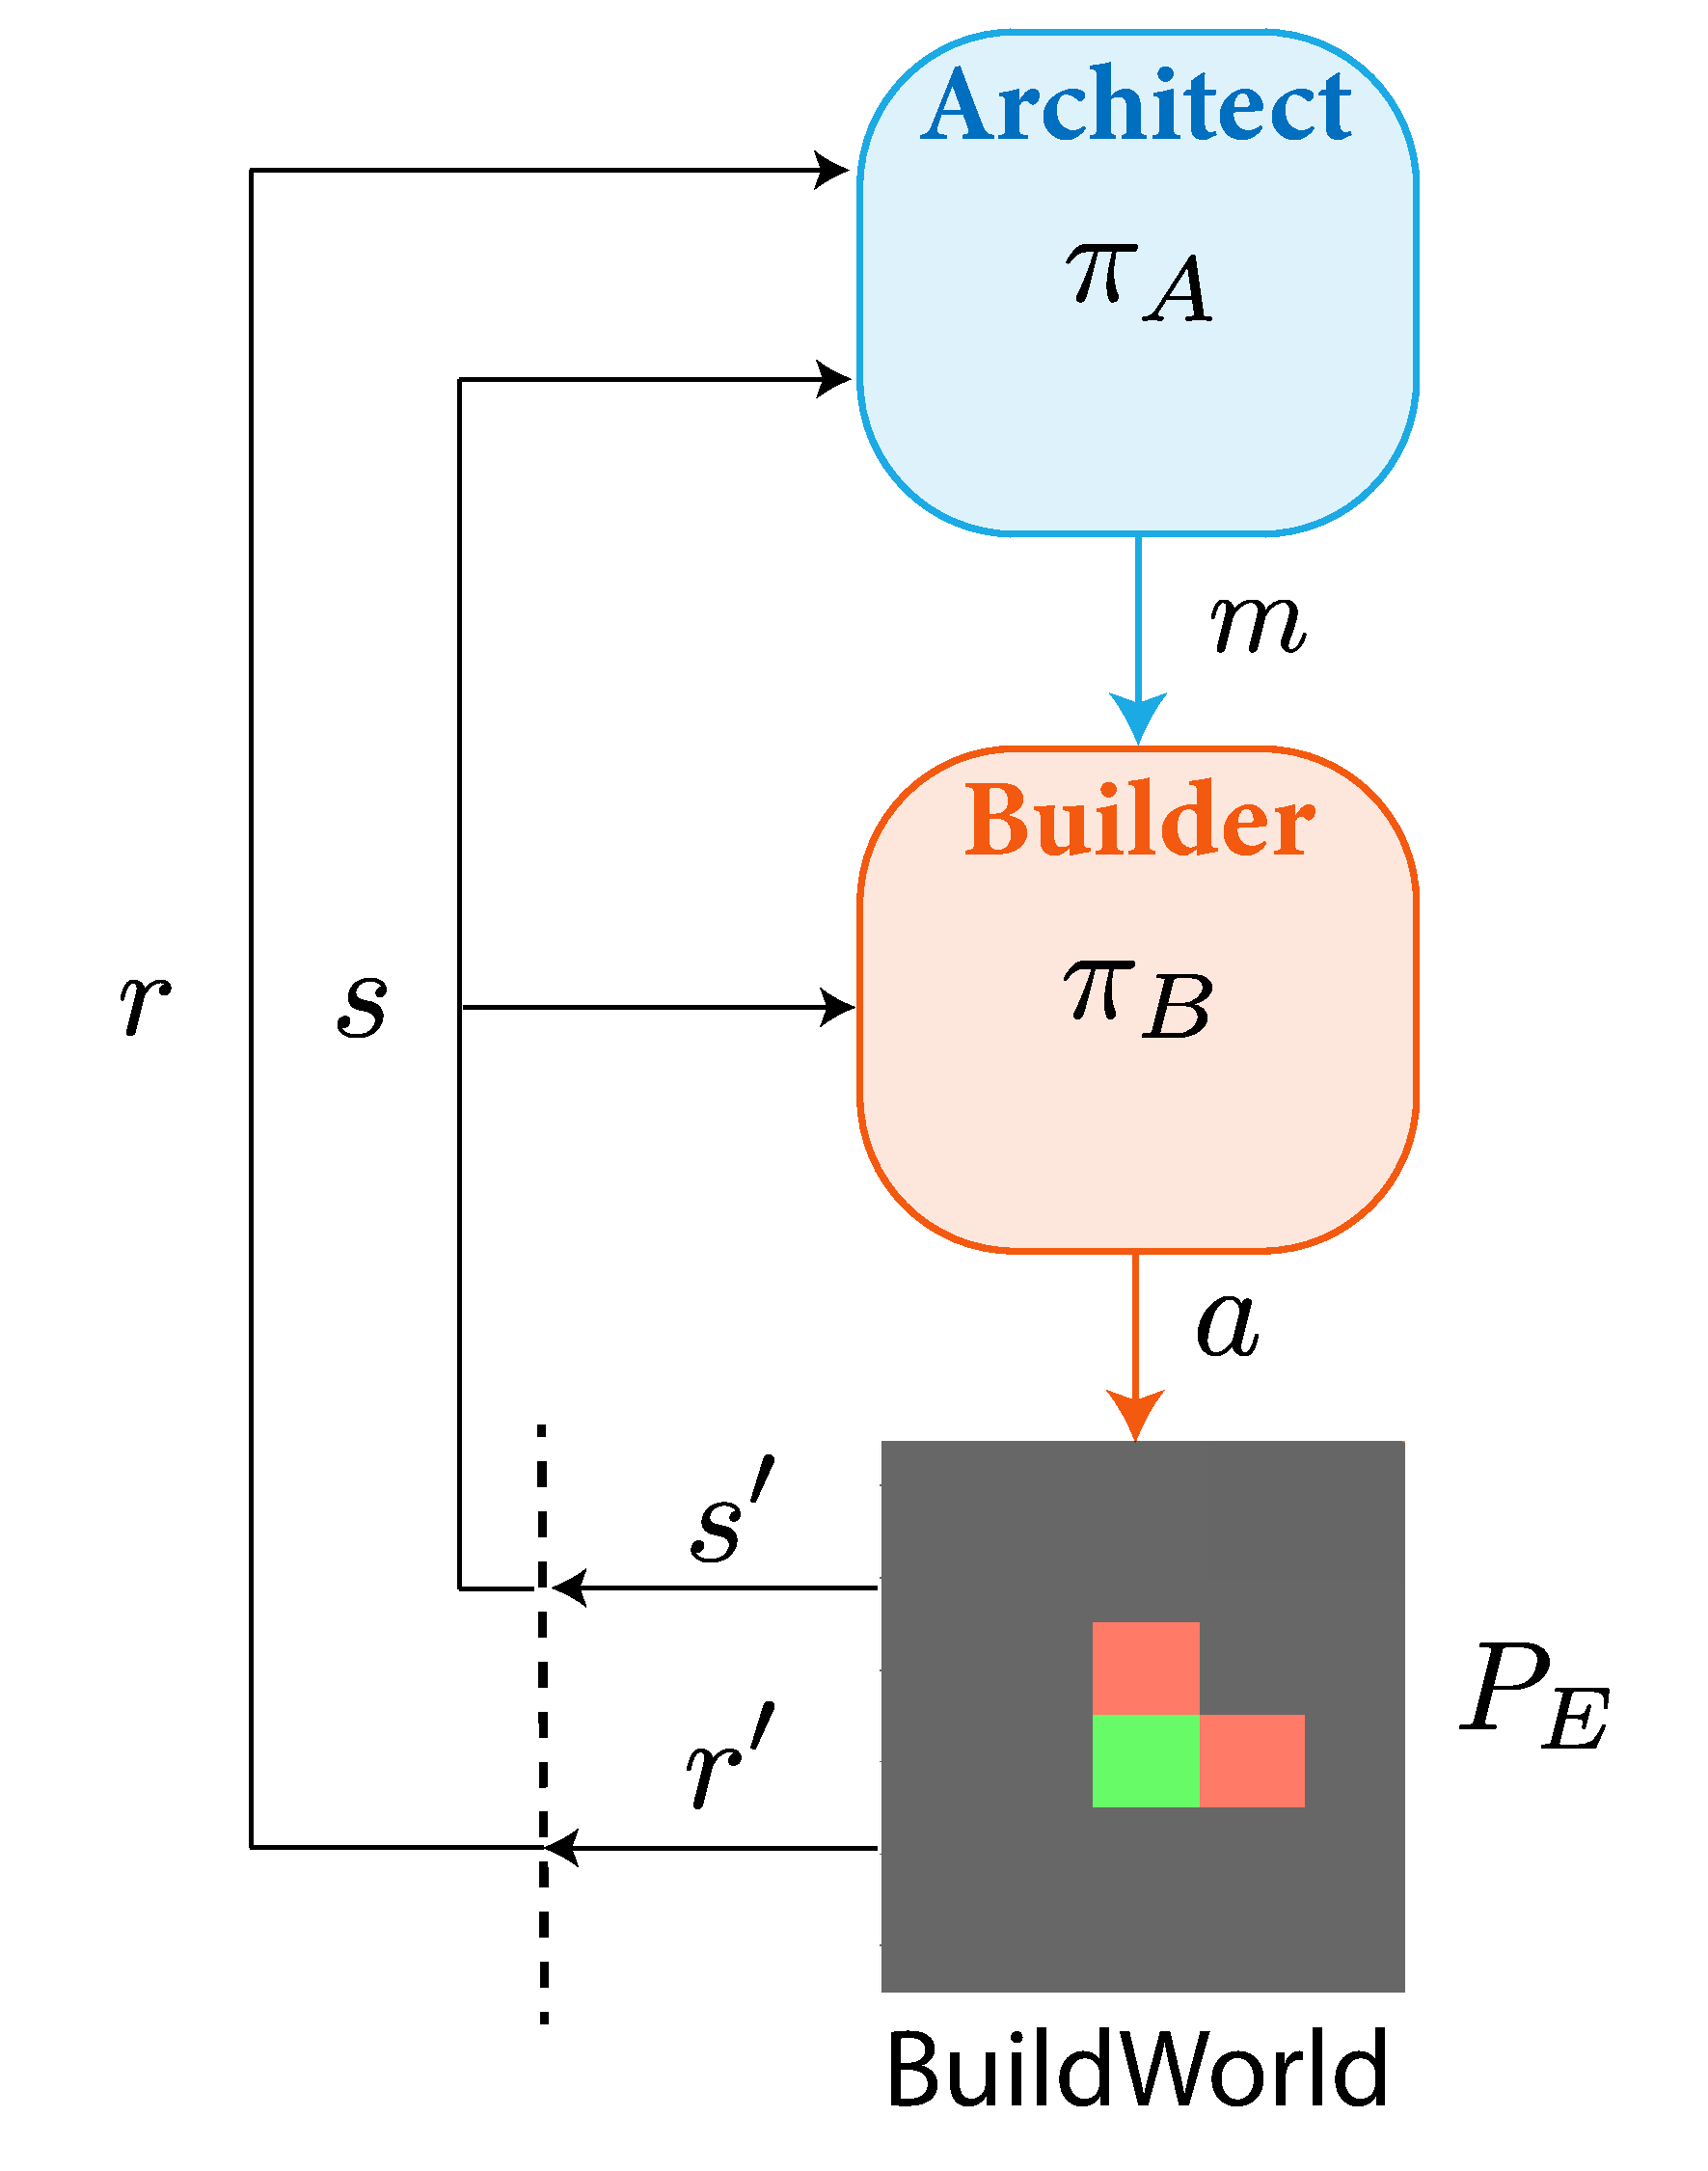
\includegraphics[width=0.22\textwidth]{abig/abp_v.pdf} & 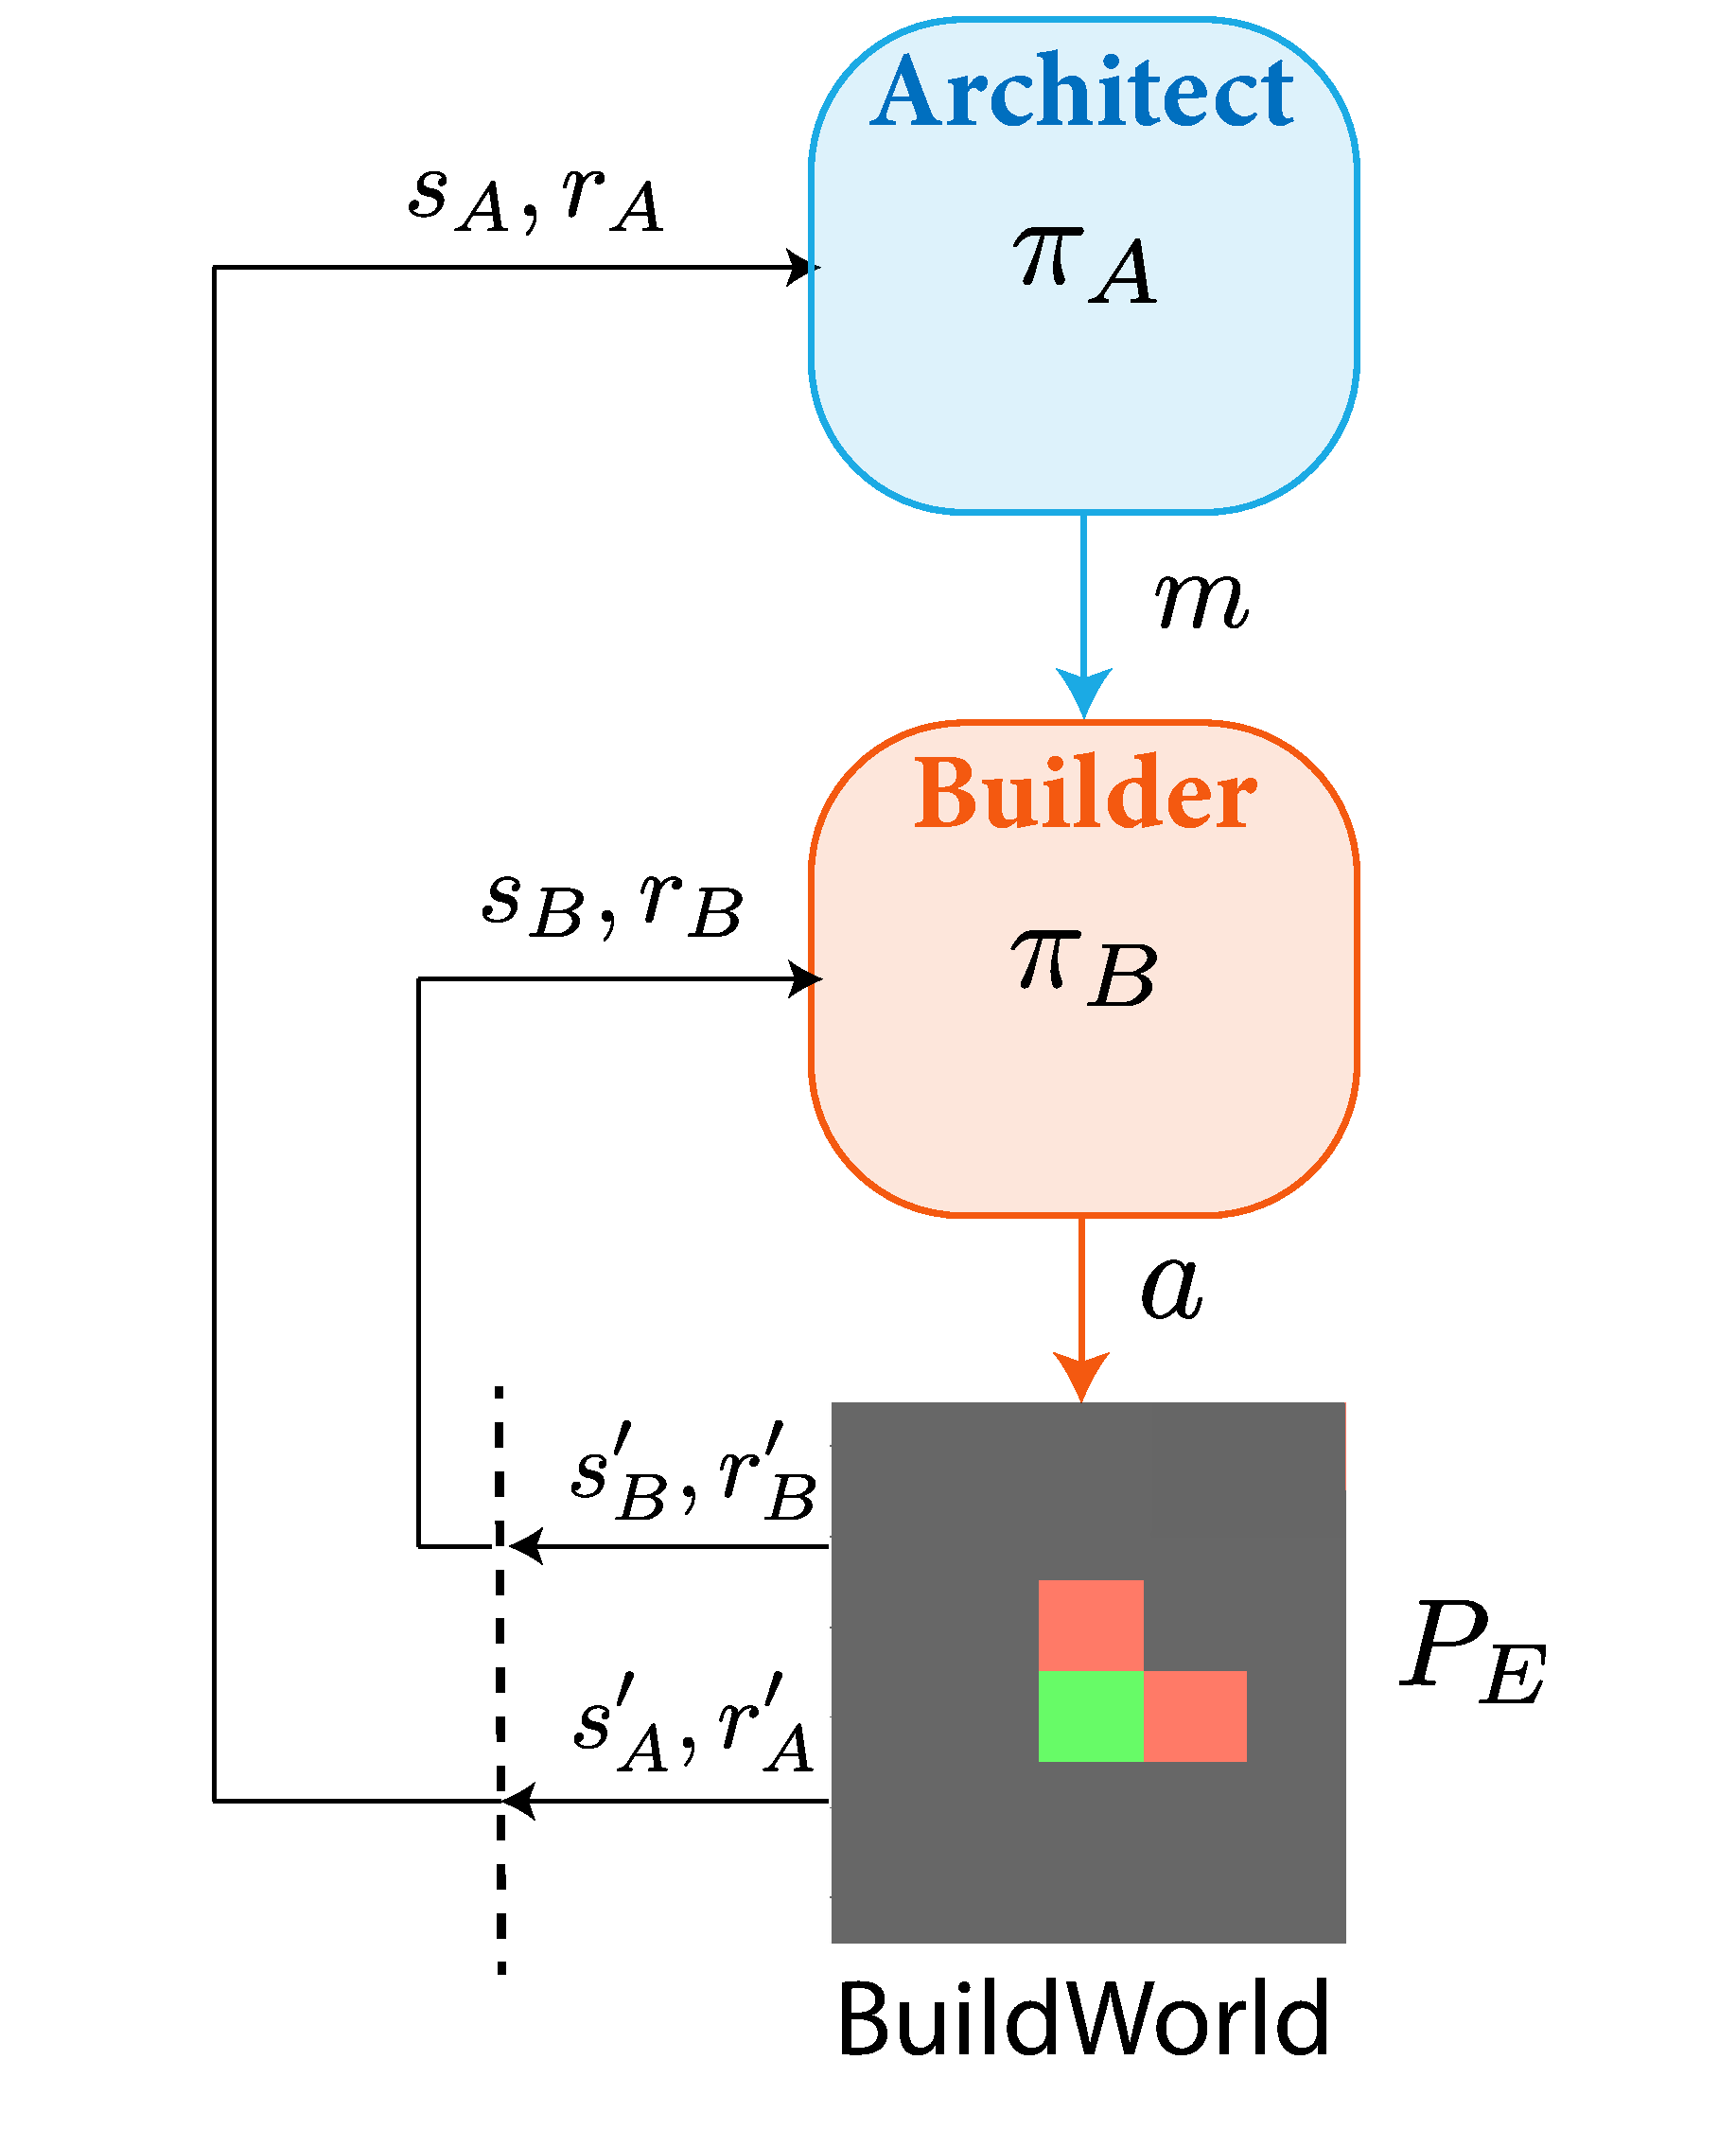
\includegraphics[width=0.23\textwidth]{abig/abp_marl.pdf} &  \multicolumn{2}{c}{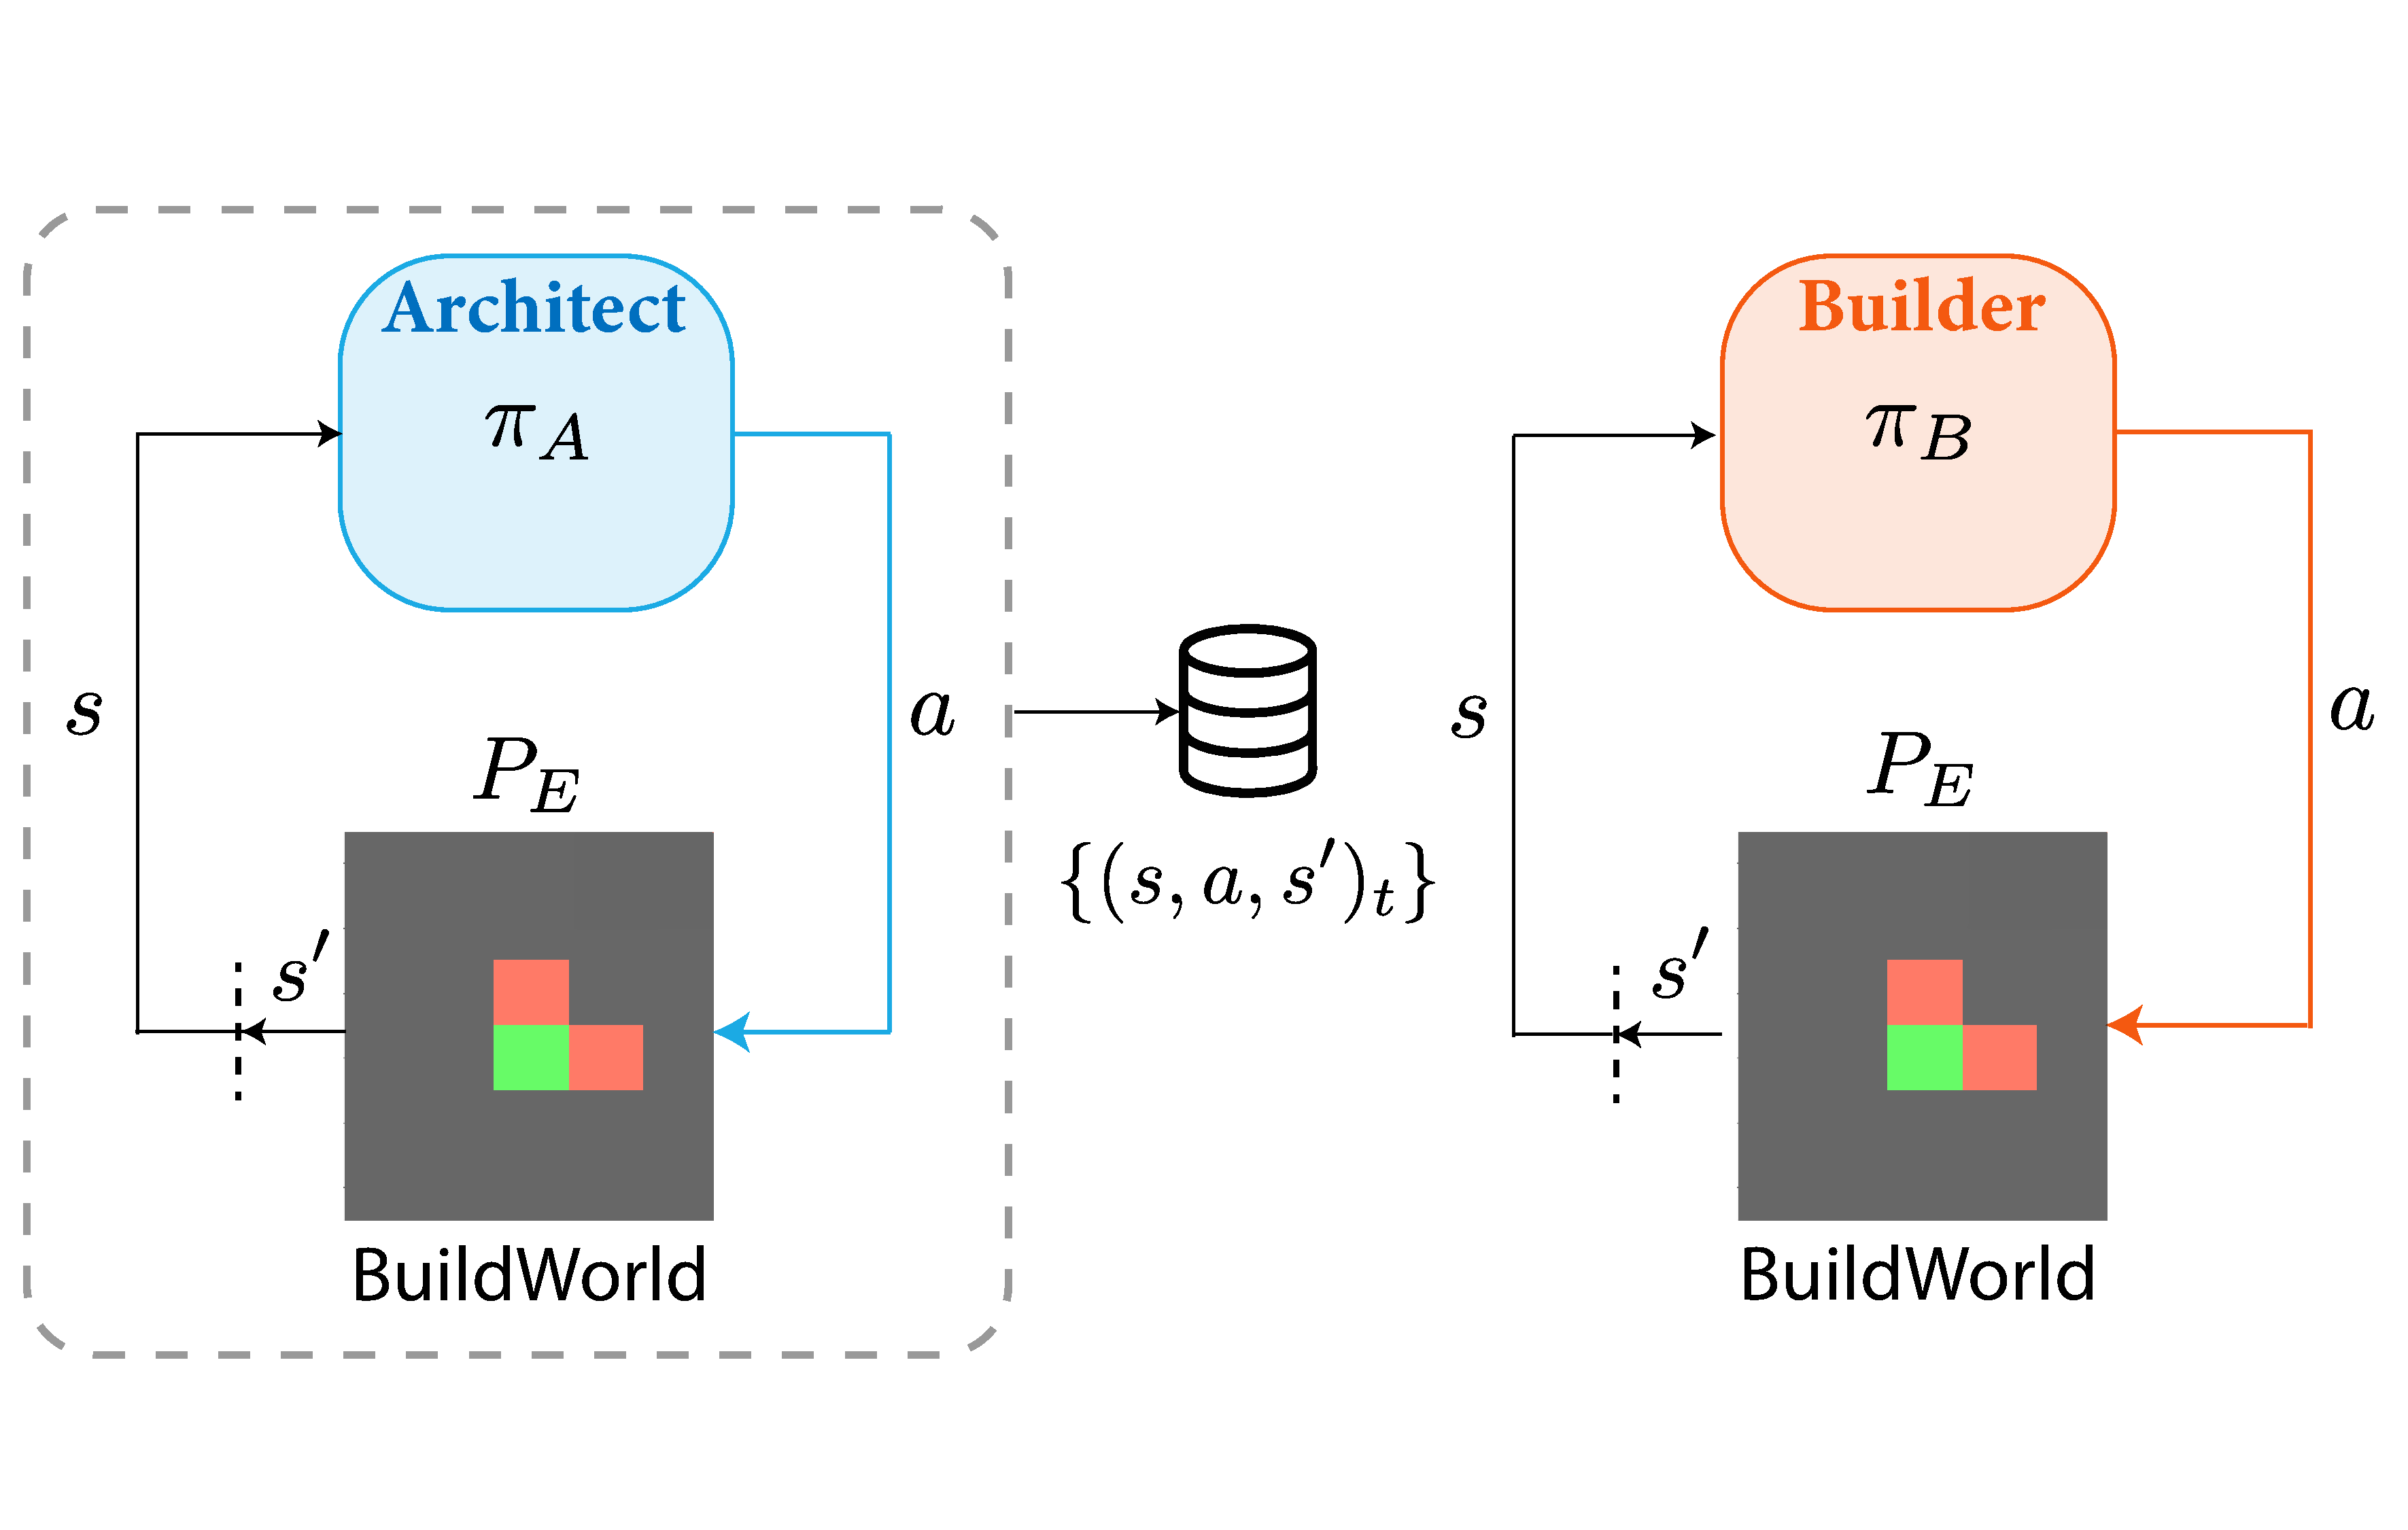
\includegraphics[width=0.46\textwidth]{abig/abp_irl.pdf}}\\
    \small (a) & \small(b) & \multicolumn{2}{c}{\small(c)}
    \end{tabular}
    \caption{\small (a) \textbf{Vertical view of the interaction diagram between the agents and the environment in our proposed ABP. } Only the architect perceives a reward signal $r$; (b) \textbf{Interaction diagram for a standard MARL modelization. } Both the architect and the builder have access to environmental rewards $r_A$ and $r_B$. Which would contradict the fact that the builder ignores everything about the task at hand; (c) \textbf{Inverse Reinforcement Learning modelization of the ABP. } The architect needs to provide demonstrations. The architect does not exchange messages with the builder. The builder relies on the demonstrations $\{(s,a,s')_t\}$ to learn the desired behavior.}
    \label{fig:sup_mdp_diag}
\end{figure}

\subsection{Analytical Description}
\label{ap:method_analytic}
\paragraph{Transition Probabilites from the architect point of view}
Using the laws of total probabilities and conditional probabilities we have: 
\begin{equation}
    \begin{split}
        \Pa(s'|s,m) &= \sum_{a\in\gA} P(s',a | s,m)\\ 
        &= \sum_{a\in\gA} P(s'|a,s,m) P(a|s,m)\\
        &= \sum_{a\in\gA} \Pe(s'|a,s) \tilde{\pi}_b(a|s,m)
    \end{split}
\end{equation}
Where the final equality uses the knowledge that next-states only depends on states and builder's actions. 

\paragraph{Reward function from the architect point of view}
\begin{equation}
    \begin{split}
        \ra(s,m,s') &\triangleq \E[R|s,m,s']\\
        &= \int_{\R}r P(r|s,m,s')dr \\
        &= \int_{\R} r\sum_{a\in\gA}P(r,a|s,m,s')dr\\
        &= \int_{\R} r\sum_{a\in\gA}P(r|s,m,a,s')P(a|s,m,s')dr\\
        &= \int_{\R} r\sum_{a\in\gA}P(r|s,a,s')\tilde{\pi}_b(a|s,m)dr\\
        &= \sum_{a\in\gA}\tilde{\pi}_b(a|s,m)\int_{\R}rP(r|s,a,s')dr\\
        &= \sum_{a\in\gA}\tilde{\pi}_b(a|s,m)r(s,a,s')
    \end{split}
\end{equation}

\paragraph{Transition function from the builder point of view}
\begin{equation}
    \begin{split}
        P(s',m'|s,m,a) &= P(m'|s',s,m,a)P(s'|s,m,a)\\
        &= P(m'|s')P(s'|s,a)\\
        &= \tildepia(m'|s') \Pe(s'|s,a)
    \end{split}
\end{equation}

\subsection{Practical Algorithm}
\label{ap:abig_algo}

\paragraph{Behavioral Cloning } 
The data-set is split into training (70\%) and validation (30\%) sets. If the validation accuracy does not improve during a \emph{wait for} number of epochs the training is early stopped. For a training data-set $\gD = \{(s,m,a)\}$ of size $N$ the BC loss to minimize for a policy $\pi_\theta$ parametrized by $\theta$ is given by: 
\begin{equation}
    J(\theta) = \frac{1}{N}\sum_{\gD}-\log\pi_\theta(a|s,m) 
\end{equation}

\paragraph{Monte-Carlo Tree Search }
In the architect's MCTS, nodes are labeled by the environment's states and they are expanded by selecting messages. Selecting message $m$ from a node with label $s$ yields a builder action according to the architect's builder model $a\sim \tildepib(a|s,m)$, this sampled action in turn yields the label of the child node according to the environment's transition model $s'\sim \Pe(s'|s,a)$. We repeat this process until we select a message that was never selected from the current node or we sample a next state that does not correspond to a child node yet. In both of these cases, a new node has to be created. We estimate the value of the new node using an engineered heuristic that estimates the return of an optimal policy $\pi^*(a|s)$ from state $s$. This value is scaled down by a factor of 2 to avoid overestimation: the builder's policy may not allow the architect to have it follow $\pi^*$. This estimated value for a newly created node at depth $l$ is back-propagated as a return to the parents node at depth $k$ according to:

\begin{equation}
    G^k=\sum_{\tau=0}^{l-1-k}\gamma^\tau r_{k+1+\tau} + \gamma^{l-k}v^l \qquad k=l,...,0
\end{equation}
where $r_j$ is the reward collected from node at depth $j$ to child node at depth $j+1$.  
From a node with label $s$ we select messages according to the Upper Confidence Bound rule: 
\begin{equation}
\label{eq:ucb}
\begin{split}
&m = \argmax_m Q(s,m) + c \sqrt{\frac{\ln \sum_b N(s,b)}{N(s,m)}}\\
&Q(s,m) = \frac{\sum_iG_i(s,m)}{N(s,m)}
\end{split}
\end{equation}
where $N(s,m)$ is the number of times message $m$ was selected from the node, $G_i(s,m)$ are the returns obtained from the node when selecting $m$ and $c$ is a constant set to $\sqrt{2}$.
When the architect must choose a message from the environment state $s$, its policy $\pia(m|s)$ runs the above procedure from a root node labeled with the current environment state $s$. After expanding a budget $b$ of nodes the architect picks the best message to send according to Eq.~(\ref{eq:ucb}) applied to the root node. It is then possible to reuse the tree for the next action selection or to discard it, if a tree is reused its maximal depth should be constrained.

\paragraph{Hyper-parameters}\textbf{ }
\begin{table}[h!]
    \centering
    \begin{tabular}{ccccc}
         sampling temperature & samples per iteration & learning rate & number of epochs & batch size\\
         \hline 
         0.5 & 100 & 0.1 & 1000 & 50
    \end{tabular}
    \caption{Toy experiment hyper-parameters}
\end{table}


\begin{table}[h!]
    \centering
    \begin{tabular}{ccc}
         budget & reuse tree & max tree depth \\
         \hline
         100 & true & 500  
    \end{tabular}
    \caption{MCTS parameters}
\end{table}

% \begin{table}[h!]
%     \centering
%     \begin{tabular}{cccc}
%         episode len & grid size & reward & message \\
%         \hline
%          40 & (5,6) & sparse & one-hot \\
%          \\
%          discount factor & episodes per interaction step & vocab size & evaluation episode len\\
%          \hline
%          0.95 & 600 & 18& 40
%     \end{tabular}
%     \caption{BuildWorld parameters (except for `6-block-shape')}
%     \label{tab:my_label}
% \end{table}

\begin{table}[h!]
    \centering
    \begin{tabular}{cccc}
        episode len & grid size & reward & message \\
        \hline
         40 & 5$\times$6 / ($6\times6$) & sparse & one-hot \\
         \\
         discount factor & episodes per iteration & vocab size & evaluation episode len\\
         \hline
         0.95 & 600 & 18 / (72) & 40 / (60)
    \end{tabular}
    \caption{BuildWorld parameters for 3 blocks / (for 6 blocks if different)}
\end{table}

% \begin{table}[h!]
%     \centering
%     \begin{tabular}{cccc}
%         grid size & vocab size & evaluation episode len \\
%         \hline
%          (6,6) & 72 & 60
%     \end{tabular}
%     \caption{BuildWorld parameters variation for `grasp' with 6 blocks}
%     \label{tab:my_label}
% \end{table}

\begin{table}[h!]
    \centering
    \begin{tabular}{cccc}
         learning rate & number of epochs  & batch-size & wait for \\
         \hline
         $5\times10^{-4}$ & 1000 & 256 & 300
    \end{tabular}
    \caption{Architect's BC parameters on BuildWorld for 3 blocks / (for 6 blocks if different)}
\end{table}

\begin{table}[h!]
    \centering
    \begin{tabular}{cccc}
         learning rate & number of epochs  & batch-size & wait for \\
         \hline
         $1\times10^{-4}$ & 1000 & 256 & 300
    \end{tabular}
    \caption{Builder's BC parameters on BuildWorld for 3 blocks / (for 6 blocks if different)}
\end{table}
Sparse reward means that the architect receives 1 if the goal is achieved and 0 otherwise. Episodes per iterations are equally divided into the modelling and guiding frames. Only the learning rates on BuildWorld were searched over with grid-searches. For BuildWorld with 3 blocks the searched range is $[ 5\times10^{-4}, 1\times10^{-4}, 1\times10^{-5}]$ for both architect and builder (vocabulary size was fixed at 6). For `grasp' with 6 blocks the searched range is $[ 1\times10^{-3}, 5\times10^{-4}, 1\times10^{-4}]$ for the architect and $[ 5\times10^{-4}, 1\times10^{-4}, 5\times10^{-5}]$ for the builder (vocabulary size was fixed at 72). The other hyper-parameters do not seem to have a major impact on the performance provided that:
\begin{itemize}[noitemsep]
    \item the MCTS hyper-parameters enable an agent that has access to the reward to solve the task.
    \item there is enough BC epochs to approach convergence.
\end{itemize}Regarding the vocabulary size, the bigger the better (see experiments in Figure~\ref{fig:dict_size_performance}). 

\paragraph{Computing resources}

A complete \abig training can take up to 48 hours on a single modern CPU (\texttt{Intel E5-2683 v4 Broadwell @ 2.1GHz}). The presented results require approximately 700 CPU hours. For each training, the main computation cost comes from the MCTS planning during the guiding frames. The self-imitation and behavior modelling steps only account for a small fraction of the computation. 
% \begin{table}[h!]
%     \centering
%     \begin{tabular}{cc}
%          architect bc learning rate & builder bc learning rate \red{to change with true value}\\
%          \hline
%          $5\times10^{-5}$ & $5\times10^{-5}$
%     \end{tabular}
%     \caption{Parameters variation for `grasp' with 6 blocks}
%     \label{tab:my_label}
% \end{table}


\newpage

\subsection{Related Work}
\label{ap:sec_related_work}
In this section we develop the differences between \abp and Hierarchical/Feudal Reinforcement Learning more in detail.

\cite{kulkarni2016hierarchical} proposes to decompose a RL agent into a two-stage hierarchy with a meta-controller (or manager) setting the goals of a controller (or worker). The meta-controller is trained to select sequences of goals that maximize the environment reward while the controller is trained to maximize goal-conditioned intrinsic rewards. The definition of the goal-space as well as the corresponding hard-coded goal-conditioned reward functions are task-related design choices. In \cite{vezhnevets2017feudal}, the authors propose a more general approach by defining goals as embeddings that directly modulate the worker's policy. Additionally, the authors define intrinsic rewards as the cosine distance between goals and embedded-state deltas (difference between the embedded-state at the moment the goal was given and the current embedded-state). Thus, goals can be interpreted as directions in embedding space.
\cite{nachum2018data} build on a this idea but let go of the embedding transformation by considering goals as directions to reach and rewards as distances between state deltas and goals. 
These works tackle the single-agent learning problem and therefore allow the manager to directly influence the learning signal of the workers. However, in the multi-agent setting where agents are physically distinct, it is not possible for an agent to explicitly tweak another agent's learning algorithm. Instead, agents must communicate by influencing each other's observations instead of intrinsic rewards. Since it is designed to investigate the emergence of communication between agents, \abp lies in this latter multi-agent setting where agents can interact with one-another only through observations. This makes applying Feudal or Hierarchical methods to the \abp unfeasible as they are restricted to worker agents that directly receive rewards. In contrast, in \abp, the reward-less builder observes communication messages that, initially, have arbitrary meaning.  




\end{document}
